\section{%
    Einführung in dynamische Systeme%
}

\subsection{%
    Was ist Kontrolltheorie?%
}

\textbf{Rückführung (feedback)}:
Bei dynamischen Systemen ändern sich die Variablen im Lauf der Zeit, oft durch externe Einflüsse.
Bei einer sog. \begriff{Rückführung (feedback)} sind mehrere dynamische Systeme miteinander
verbunden und beeinflussen sich gegenseitig.

\textbf{Beispiele}:
\begin{itemize}
    \item
    Knopf zur automatischen Geschwindigkeitsreglung in US-amerikanischen Autos

    \item
    Biologie: z.\,B. die Regulierung des Glukosespiegels im Blut, damit dieser konstant bleibt
    (Leber und Pankreas messen bzw. schütten die Hormone Insulin und Glukagon aus und beeinflussen
    sich somit gegenseitig)

    \item
    \begriff{Steuerproblem}: Flug einer Rakete zum Mond mit möglichst wenig Treibstoffaufwand

    \item
    \begriff{Fliehkraftregler (centrifugal governor)}:
    Dieser hält die Rotationsgeschwindigkeit auf einem konstanten Wert,
    der von der Belastung der Maschine unabhängig ist.
    Obwohl er seit dem 17. Jahrhundert bekannt ist, wird er meist Watt/Boulton
    (1788) zugeschrieben.
    Eine theoretische Stabilitätsanalyse wurde von Maxwell und Hurwitz durchgeführt.
    Man spricht von negativer Rückführung, da das Ventil geschlossen/geöffnet wird,
    wenn sich die Maschine zu schnell/zu langsam bewegt.
    Allerdings muss nicht ein stabiles Gleichgewicht eintreten,
    es wäre z.\,B. auch eine Oszillation möglich
    (wie die Temperatur beim Thermostat).
\end{itemize}

\linie

\textbf{positive Auswirkungen von Rückführung}:
\begin{itemize}
    \item
    Erhöhung der Unempfindlichkeit des Systems auf externe Einflüsse\\
    (mehr Glukose durch Essen, Änderung der Belastung beim Fliehkraftregler)

    \item
    Erhöhung der Robustheit gegen Veränderungen in den Komponenten\\
    (Veränderung der Masse des Rades beim Fliehkraftregler)

    \item
    lineares Verhalten bei nicht-linearen Systemen erzwingen\\
    (Autopilot bei Kampfjets, Leistungselektronik)
\end{itemize}

\textbf{negative Auswirkungen von Rückführung}:
\begin{itemize}
    \item
    Erzeugung von dynamischen Instabilitäten, also Oszillationen oder bestimmte Divergenz\\
    (Reduktion der Reibung durch Optimierung der Maschine kann zu Oszillationen beim
    Fliehkraftregler führen)

    \item
    Erhöhung der Empfindlichkeit auf externe Einflüsse und Veränderungen der Komponenten\\
    (Verstärkung des Rauschens bei einem Sensor)
\end{itemize}

\linie

\textbf{Kontrolltheorie}:
Der Zweck von \begriff{Regelung (control)} ist die Gestaltung von Komponenten eines
technischen Rückführungssystems, um ein gewünschtes Gesamtverhalten zu erzielen.\\
\begriff{Kontrolltheorie (control theory)} stellt die notwendigen mathematischen Grundlagen,
Werkzeuge und Algorithmen sowie das nötige Vokabular bzw. die Technik bereit, um dieses Ziel zu
erreichen.

\pagebreak

\subsection{%
    Mathematische Modelle dynamischer Systeme%
}

\textbf{dynamisches System}:\\
In einem \begriff{dynamischen System} treten die Auswirkungen einer Aktion nicht sofort auf.

Zum Beispiel erhöht die Betätigung des Gaspedals im Auto nicht sofort die Geschwindigkeit,
die Temperatur steigt nicht sofort an, wenn die Heizung angeschaltet wird,
Kopfschmerzen verschwinden erst langsam, nachdem Medizin eingenommen wurde, und
eine Geldanlage führt nur in der Zukunft zu Gewinnen oder Verlusten.

Variablen eines dynamischen Systems verändern sich mit der Zeit.
Die Entwicklung hängt dabei von der äußeren Anregung ab, die sich selbst mit der Zeit ändert.

\linie

\textbf{mathematisches Modell}:
Eine Möglichkeit der Analyse des Verhalten eines dynamischen Systems besteht mittels eines
\begriff{mathematischen Modells}.
Solche Modelle werden oft durch (gewöhnliche oder partielle)
\begriff{Dif"|ferentialgleichungen} beschrieben.

\textbf{Beispiel}:
Beim \begriff{gedämpften Federpendel (mass-spring-damper system)} hängt eine Masse $m$ mittels
einer Feder (Federkonstante $k$) an einer Wand (Abstand $q$, abhängig von der Zeit $t$).
Gleichzeitig ist zwischen Masse und Wand eine Dämpfung $c(\dot{q})$ eingebaut, die von der
Geschwindigkeit der Masse abhängt (auch nicht-linear möglich).
Nach dem zweiten Newtonschen Gesetz und dem Hookeschen Gesetz gilt
$m \ddot{q} + c(\dot{q}) + kq = 0$
(Federkraft wirkt in Richtung der Ruheposition).

\linie

\textbf{Eingangsgrößen}:
Ein dynamisches System ist \begriff{autonom (autonomous)},
falls es nicht externen Einflüssen ausgesetzt ist.
Nicht-autonome Systeme haben externe \begriff{Eingangsgrößen (inputs)}.

\textbf{Beispiel}:
Im obigen Beispiel erhält man mit $u(\cdot)$ der externen Kraft, die auf die Masse wirkt,
$m \ddot{q} + c(\dot{q}) + kq = u$.
Die Kraft $u(\cdot)$ variiert normalerweise mit der Zeit.
Je nach Umständen kann sie auf zwei verschiedene Arten interpretiert werden:
\begin{itemize}
    \item
    \begriff{Steuergröße (control input)}:
    falls $u(\cdot)$ frei verändert werden darf

    \item
    \begriff{Störgröße (disturbance input)}:
    falls $u(\cdot)$ durch die Natur feststeht und nicht verändert werden darf
\end{itemize}

\linie

\textbf{Ausgangsgrößen}:
Meistens interessiert man sich nicht für alle Variablen, die in einem Modell vorkommen.
\begriff{Ausgangsgrößen (outputs)} beschreiben die Größen, für die man sich interessiert.

\textbf{Beispiel}:
Wenn man sich im obigen Beispiel nur für die Auslenkung interessiert, dann ist der
Ausgang $y$ bestimmt durch $m \ddot{q} + c(\dot{q}) + kq = u$, $y = q$.
Für eine bestimmte Steuergröße $u(\cdot)$ ist die Ausgangsgröße $y(\cdot)$ eine Funktion in
Abhängigkeit von der Zeit.
Auch $y$ kann auf zwei Arten interpretiert werden:
\begin{itemize}
    \item
    $y$ ist eine Variable, die gemessen werden kann (mittels Sensoren).

    \item
    $y$ ist eine Variable, die zur Analyse der Eigenschaften des Systems überwacht werden soll
    (in der Simulation).
\end{itemize}

\linie
\pagebreak

\textbf{Interpretation des Modells}:
Seien $u(t)$ eine Eingangsgröße, die für $t \ge 0$ definiert ist, und
$q_0$ und $v_0$ eine Anfangsposition bzw. eine Anfangsgeschwindigkeit.
Falls $u \in \C$ und $c \in \C^1$ gilt,
dann hat das Anfangswertproblem $m \ddot{q}(t) + c(\dot{q}(t)) + k q(t) = u(t)$ mit $q(0) = q_0$,
$\dot{q}(0) = v_0$ eine eindeutige, dif"|ferenzierbare Lösung $q(t)$, die für $t \in [0, t_1)$
mit einem $t_1 > 0$ definiert ist
(die Lösung muss nicht für alle $t \ge 0$ existieren).

\textbf{Zustandsgröße}:
Weil die Werte für $q(0)$ und $\dot{q}(0)$ die Lösung der DGL (für eine feste Eingangsgröße)
eindeutig festlegen,
heißen $x = \smallpmatrix{x_1 \\ x_2} := \smallpmatrix{q \\ \dot{q}}$ und
$x(t) = \smallpmatrix{x_1(t) \\ x_2(t)} := \smallpmatrix{q(t) \\ \dot{q}(t)}$
\begriff{Zustandsvektor (state-vector)} bzw. \begriff{Zustandsgröße (state-response)}.
Der \begriff{Ausgang (response)} des Systems ist bestimmt durch $y(t) = q(t)$.

\textbf{Verhalten}:
Bei einem System wie $m \ddot{q} + c(\dot{q}) + kq = u$, $y = q$
ist man an seinem \begriff{Verhalten (behavior)} interessiert,
also die Menge aller Eingangs-, Zustands- und Ausgangsgrößen $u(\cdot)$,
$(q(\cdot), \dot{q}(\cdot))$ und $y(\cdot)$, die diese Gleichung erfüllen.

\textbf{Trajektorien}:
\begriff{Signale (signals)} oder \begriff{Traktorien (trajectories)}
sind vektorwertige Funktionen der Zeit.
Normalerweise wird stillschweigend angenommen, dass sie abschnittsweise stetig sind.

Die Bedingungen, die erfüllt sein müssen, werden oft durch DGLs beschrieben.
Dabei müssen Annahmen gemacht werden, sodass die Existenz und Eindeutigkeit der Lösung des
Anfangswertproblems sichergestellt ist.

\textbf{Äquivalenz}:
Verschiedene Beschreibungen eines Systems können zum selben Verhalten führen.
In diesem Fall heißen die System(-Beschreibungen) \begriff{äquivalent (equivalent)}.
Im sog. \begriff{verhaltens"-basierten Ansatz} bei dynamischen Systemen wird die nötige Theorie in
einer mathematisch präzisen Weise entwickelt.

\linie

\textbf{beispielhafte Fragen}:
\begin{itemize}
    \item
    Falls es keinen externen Einfluss gibt, wie verhalten sich die Zustands- und Ausgangsgröße?

    \item
    Kann das System von einer Position in eine andere gebracht werden
    (\begriff{Steuerproblem, steering problem})?

    \item
    Ist es möglich, die Eingangs- aus der Ausgangsgröße zu rekonstruieren?

    \item
    Kann das System so modifiziert werden, sodass ein gewünschtes Verhalten erzielt wird?
\end{itemize}
Bei manchen von diesen (groben) Fragen muss das System auf seine Eigenschaften hin untersucht
werden, bei anderen müssen Eingangsgrößen verarbeitet oder die Systembedingungen verändert werden,
um das Verhalten des Systems zu ändern.
Mit der Kontrolltheorie versucht man, solche Fragen systematisch zu beantworten.

\linie
\pagebreak

\textbf{von Modellen zweiter zu Modellen erster Ordnung}:
Die Beschreibung $m \ddot{q} + c(\dot{q}) + kq = u$ beinhaltet die ersten beiden
Ableitungen von $q$.
Für $m \not= 0$ heißt sie \begriff{DGL zweiter Ordnung}.
Mit den \begriff{Zustandsvariablen (state-variables)} $x_1 = q$ und $x_2 = \dot{q}$
gilt $\dot{x}_1 = \dot{q} = x_2$, also\\
$\dot{x}_2 = \ddot{q} = -\frac{k}{m} q - \frac{c(\dot{q})}{m} + \frac{1}{m} u
= -\frac{k}{m} x_1 - \frac{1}{m} c(x_2) + \frac{1}{m} u$.
Das kann geschrieben werden als\\
$\dot{x} := \smallpmatrix{\dot{x}_1 \\ \dot{x}_2}
= \smallpmatrix{x_2 \\ -\frac{k}{m} x_1 - \frac{1}{m} c(x_2) + \frac{1}{m} u}
=: f(x, u)$,
man erhält also eine zweidim. \begriff{DGL erster Ordnung}.

\textbf{Lemma (Umwandlung in System erster Ordnung)}:
Sei $r$ eine reellwertige, nicht-lineare Funktion mit $n + 1$ Argumenten.
Dann ist das System
$q^{(n)} + r(q^{(n-1)}, q^{(n-2)}, \dotsc, \dot{q}, q, u) = 0$
äquivalent zu
$\dot{x} := \smallpmatrix{\dot{x}_1 \\ \dot{x}_2 \\ \vdots \\ \dot{x}_{n-1} \\ \dot{x}_n}
= \smallpmatrix{x_2 \\ x_3 \\ \vdots \\ x_n \\ -r(x_n, x_{n-1}, \dotsc, x_2, x_1, u)}
=: f(x, u)$.

Diese Methode ist jedoch nicht eindeutig:

\textbf{Lemma (Umwandlung in System erster Ordnung 2)}:
Sei $r$ eine reellwertige, nicht-lineare Funktion mit $n + 1$ Argumenten.
Dann ist das System
$q^{(n)} + r(q^{(n-1)}, q^{(n-2)}, \dotsc, \dot{q}, q, u) = 0$
äquivalent zu
$\dot{z} := \smallpmatrix{\dot{z}_1 \\ \dot{z}_2 \\ \vdots \\ \dot{z}_{n-1} \\ \dot{z}_n}
= \smallpmatrix{-r(z_1, z_2, \dotsc, z_{n-1}, z_n, u) \\ z_1 \\ \vdots \\ z_{n-2} \\ z_{n-1}}
=: \widehat{f}(z, u)$.

\vspace{3mm}
\linie

\textbf{Zustandsraum-Darstellung}:
Physikalische Modelle führen oft zu einem System von DGLs höherer Ordnung.
Wie gerade gezeigt, können diese oft (aber nicht immer!) äquivalent geschrieben werden als
eine Vektor-DGL erster Ordnung
$\dot{x} = f(x, u)$ und $y = h(x, u)$ mit
Abbildungen $f\colon X \times U \rightarrow \real^n$ und
$h\colon X \times U \rightarrow \real^k$,
wobei $X \subset \real^n$ und $U \subset \real^m$.\\
Ausführlich geschrieben:
\begin{align*}
    \dot{x}_1 &= f_1(x_1, \dotsc, x_n, u_1, \dotsc, u_m),&
    y_1 &= h_1(x_1, \dotsc, x_n, u_1, \dotsc, u_m),\\
    &\;\;\vdots&&\;\;\vdots\\
    \dot{x}_n &= f_n(x_1, \dotsc, x_n, u_1, \dotsc, u_m),&
    y_k &= h_k(x_1, \dotsc, x_n, u_1, \dotsc, u_m).
\end{align*}
Diese Darstellung nennt man die \begriff{Zustandsraum-Darstellung (state-space description)}.
Die Funktionen können auch explizit von der Zeit abhängen.

Wenn $u(\cdot)\colon I \rightarrow U$ eine Eingangsgröße auf einem of"|fenen Intervall
$I \subset \real$ mit $0 \in I$ und $\xi \in \real^n$ eine Anfangsbedingung für den Zustand ist,
dann erhält man die Zustandsgröße durch Lösung des AWP
$\dot{x}(t) = f(x(t), u(t))$, $x(0) = \xi$.
Die Ausgangsgröße ist dann einfach $y(t) := h(x(t), u(t))$ für $t \in I$.

Die Existenz und Eindeutigkeit der Zustandsgröße $x$ auf einem of"|fenen Teilintervall von $I$
ist garantiert, wenn $f$ stetig in $(x, u)$,
$f$ Lipschitz-stetig in $x$ und $u$ stetig ist.
Das gilt auch für Eingänge $u$, die nur abschnittsweise stetig sind (endlich viele Sprungstellen).
In diesem Fall löst man die DGL abschnittsweise und setzt als Anfangsbedingung für
den zweiten Abschnitt den Wert der Lösung im ersten Abschnitt an der Zeit ein, an der
der Sprung stattfindet.
Dadurch ist die Lösung in jedem Fall stetig, wird jedoch Sprünge in der Ableitung besitzen.

\linie

\textbf{allgemeine Beschreibung eines linearen Systems}:
Wenn $f$ und $h$ linear sind, dann gilt
$f(x, u) = Ax + Bu$ und $h(x, u) = Cx + Du$
mit $A \in \real^{n \times n}$, $B \in \real^{n \times m}$, $C \in \real^{k \times n}$,
$D \in \real^{k \times m}$.\\
Daher wird ein allgemeines lineares, zeit-invariantes System,
genannt \begriff{LTI-System (linear, time-\\invariant system)}, beschrieben durch
$\dot{x} = Ax + Bu$, $y = Cx + Du$.

Dieses System wird im Folgenden hauptsächlich verwendet,
denn viele technische Systeme können oft durch lineare Systeme angenähert werden.
Andererseits benötigen physikalische Modelle oft nicht-lineare dynamische Systeme.

\pagebreak

\subsection{%
    \emph{Wiederholung}: Globale Existenz und Eindeutigkeit von Lösungen von Anfangswertproblemen%
}

Sei das Anfangswertproblem $\dot{x} = g(t, x)$, $x(\tau) = \xi$,
für $g\colon D \rightarrow \real^n$ mit $D \subset \real \times \real^n$ gegeben.

\textbf{Voraussetzungen}:
Seien $D \subset \real \times \real^n$ of"|fen und $g\colon D \rightarrow \real^n$
stetig in $(t, x)$ und\\
\begriff{lokal \name{Lipschitz}-stetig} in $x$, d.\,h.
für alle $(\tau, \xi) \in D$ gibt es eine Umgebung $U \subset D$ von $(\tau, \xi)$
und ein $L > 0$ mit
$\norm{g(t, x) - g(t, y)} \le L \norm{x - y}$ für alle $(t, x), (t, y) \in U$.

Die Voraussetzungen sind erfüllt, wenn $g$ und $\partial_x g$ stetig auf $D$ sind,
also insbesondere, wenn $g \in \C^1(D, \real^n)$.

\linie

\textbf{Satz (globale Existenz und Eindeutigkeit)}:
Unter obigen Voraussetzungen gibt es für jedes $(\tau, \xi) \in D$ ein
maximales Existenzintervall $I_{(\tau, \xi)} = (t_-, t_+)$ mit $\tau \in I_{(\tau, \xi)}$
und eine eindeutige $\C^1$-Lösung
$x(\cdot, \tau, \xi)\colon I_{(\tau, \xi)} \rightarrow \real^n$
des AWP $\dot{x} = g(t, x)$, $x(\tau) = \xi$.\\
Maximalität von $I_{(\tau, \xi)}$ bedeutet, dass für jede $\C^1$-Lösung
$x_J\colon J \rightarrow \real^n$ des AWP auf einem Intervall $J$ mit $\tau \in J$
automatisch $J \subset I_{(\tau, \xi)}$ und $x_J = x|_J$ erfüllt ist.\\
Außerdem gilt für $t_+ < \infty$ genau eine der folgenden beiden Eigenschaften
(analog für $t_- > -\infty$):
\begin{itemize}
    \item
    Die Lösung divergiert bestimmt in der Norm:\\
    $\lim_{t \to t_+-0} \norm{x(t)} = \infty$.

    \item
    Die Lösung nähert sich dem Rand von $D$ an:\\
    Für alle Folgen $(t_\nu)_{\nu \in \natural}$ in $I_{(\tau, \xi)}$ mit
    $t_\nu \to t_+$ und $x(t_\nu) \to x_+$
    gilt $(t_+, x_+) \in \partial D$.
\end{itemize}

\pagebreak

\subsection{%
    Simulation%
}

\textbf{Integraldarstellung von DGLs}:
Die Beschreibung eines Systems mit Dif"|ferential- und Ausgangsgleichung
$\dot{x}(t) = f(x(t), u(t))$, $x(0) = \xi$, und $y(t) = h(x(t), u(t))$
erlaubt die numerische Berechnung des Ausgangs (für einen Eingang und eine Anfangsbedingung)
durch ODE-Löser wie z.\,B. \code{ode45} oder \code{ode15s} in MATLAB.
Durch Integration der DGL über die Zeit erhält man die Integraldarstellung
$x(t) = \xi + \int_0^t f(x(\tau), u(\tau))\d\tau$, $y(t) = h(x(t), u(t))$.

Die Darstellung kann man wie folgt interpretieren:
Definiere zunächst die Abbildung $\Sigma_1$ mit
$\smallpmatrix{x(\cdot) \\ u(\cdot)} \mapsto z(\cdot)$,
wobei $z(t) := f(x(t), u(t))$ (\begriff{statisches System (static system)}).
Definiere dann die Integration mit Anfangswert $\xi$:
$\Sigma_2$ mit $v(\cdot) \mapsto w(\cdot)$, wobei $w(t) := \xi + \int_0^t v(\tau)\d\tau$.
Durch Komposition der beiden Abbildungen erhält man die Abbildung $\Sigma_2 \circ \Sigma_1$ mit
$\smallpmatrix{x(\cdot) \\ u(\cdot)} \mapsto w(\cdot)$, wobei
$w(t) := \xi + \int_0^t f(x(\tau), u(\tau))\d\tau$.
Für ein festes $u(\cdot)$ ist nun ein Fixpunkt $x(\cdot)$ dieser Abbildung gesucht.
Dies kann man in einem \begriff{Simulink-Diagramm} darstellen:
\begin{center}
    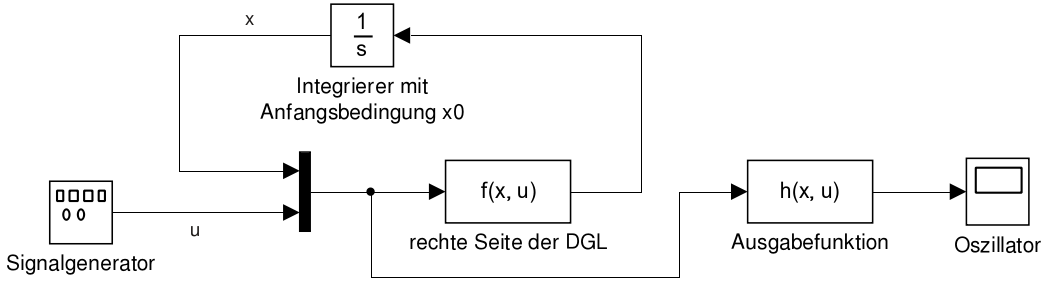
\includegraphics[scale=\modelscale]{dgl}
\end{center}
Den Ausgang erhält man dann einfach durch Anwendung von $h(\cdot, \cdot)$ auf
$x(\cdot)$ und $u(\cdot)$ (wie bei $\Sigma_1$).

\linie

\textbf{inverses Pendel}:
Ein \begriff{inverses Pendel (cart-pendulum system)} ist ein mathematisches Pendel,
das in der Ruhelage nach oben zeigt.
Das Pendel kann nur in einer Dimension schwingen und ist auf einem Wagen befestigt,
der sich in derselben Dimension hin- und her bewegen kann.
Der "`Wagen"' ist so gebaut, dass das Pendel auch nach unten schwingen kann,
es kann also die \SI{360}{\degree} voll ausnutzen.
Das Ziel ist, das Pendel durch Bewegung des Wagens in seiner instabilen Ruhelage zu halten.
Ein Segway kann vereinfacht als inverses Pendel betrachtet werden.

Bezeichnet man
die Masse am Pendel mit $m$,
die Masse des Wagens mit $M$,
die zurückgelegte Strecke des Wagens mit $p$,
die auf den Wagen wirkende Kraft mit $F$,
die Länge des Pendels mit $\ell$ und
den Winkel der Auslenkung des Pendels aus der Ruhelage mit $\theta$,
so erhält man mit den \begriff{\name{Lagrange}-Gleichungen}
$(M + m)\ddot{p} - m\ell \cos(\theta)\ddot{\theta} + c\dot{p} +
m\ell \sin(\theta)\dot{\theta}^2 = F$ sowie\\
$-m\ell \cos(\theta)\ddot{p} + m\ell^2\ddot{\theta} + \gamma \dot{\theta} -
mg\ell \sin(\theta) = 0$,
wobei $c$ und $\gamma$ den Reibungswiderstand des Wagens und des Pendels beschreiben.

Mit $U(\theta) := \smallpmatrix{M + m&-m\ell\cos(\theta)\\-m\ell\cos(\theta)&m\ell^2}$ und
$v(\theta, \dot{p}, \dot{\theta}) := \smallpmatrix{c\dot{p} + m\ell\sin(\theta)\dot{\theta}^2 \\
\gamma\dot{\theta} - mg\ell\sin(\theta)}$
kann man das System schreiben als $U(\theta) \smallpmatrix{\ddot{p} \\ \ddot{\theta}} +
v(\theta, \dot{p}, \dot{\theta}) = \smallpmatrix{F \\ 0}$.
Dabei ist $U(\theta)$ invertierbar, weil die Determinante für kein $\theta$ verschwindet.
Deswegen kann man dies schreiben als\\
$\smallpmatrix{\ddot{p} \\ \ddot{\theta}} = -U(\theta)^{-1} v(\theta, \dot{p}, \dot{\theta}) +
U(\theta)^{-1} \smallpmatrix{F \\ 0} =: \smallpmatrix{w_1(p, \theta, \dot{p}, \dot{\theta}, F) \\
w_2(p, \theta, \dot{p}, \dot{\theta}, F)}$.

Wenn man die Zustandsgrößen $\smallpmatrix{x_1 \\ x_2} := \smallpmatrix{p \\ \theta}$ und
$\smallpmatrix{x_3 \\ x_4} := \smallpmatrix{\dot{p} \\ \dot{\theta}}$
sowie die Eingangsgröße $u := F$ definiert,
so kann das System durch $\dot{x} = f(x, u)$ als System erster Ordnung beschrieben werden,
wobei $f(x, u) := \smallpmatrix{x_3 \\ x_4 \\ w_1(x, u) \\ w_2(x, u)}$.

\pagebreak

\subsection{%
    Gleichgewichte und Linearisierung%
}

\textbf{Gleichgewicht}:
Alle Paare von Vektoren $(x_e, u_e) \in X \times U$ mit $f(x_e, u_e) = 0$ heißen\\
\begriff{Gleichgewichte (equilibria)} des Systems $\dot{x} = f(x, u)$.

%Wenn ein System mit der konstanten Steuergröße $u(t) = u_e$ betrieben und
%der Zustand durch $x_e(t_0) = x_e$ initialisiert wird, so gilt für die Zustandsgröße
%$x(t) = x_e$ und $\dot{x}(t) = 0$ für alle $t \ge t_0$,
%d.\,h. wenn ein System im Gleichgewicht startet,
%dann bleibt die Zustandsgröße auch da.

Wenn ein System mit der konstanten Steuergröße $u(t) = u_e$ betrieben wird,
der Zustand durch $x_e(t_0) = x_e$ initialisiert wird und die Lösung des Systems eindeutig ist,
dann gilt $x(t) \equiv x_e$ für alle $t \ge t_0$
(weil das eine Lösung ist, da $f(x_e, u_e) = 0$).

\textbf{Beispiel}:
Für Gleichgewichte in obiger DGL müssen die Ableitungen von $p$ und $\theta$ verschwinden,
also $0 = F$ und $-mg\ell \sin(\theta) = 0$.
Die Lösungen sind $\theta_e = 0$ (aufrechte Position) und $\theta_e = \pi$ (nach unten zeigend),
wobei $p_e$ beliebig ist.

\linie

\textbf{Herleitung der Linearisierung}:
Falls $f$ und $h$ stetig dif"|ferenzierbar sind, kann man die Taylorentwicklungen erster Ordnung
um $(x_e, u_e)$ berechnen als\\
$f(x, u) \approx f(x_e, u_e) + \partial_x f(x_e, u_e) (x - x_e) +
\partial_u f(x_e, u_e) (u - u_e)$ und\\
$h(x, u) \approx y_e + \partial_x h(x_e, u_e) (x - x_e) +
\partial_u h(x_e, u_e) (u - u_e)$, wobei $y_e := h(x_e, u_e)$.\\
Dabei sind die partiellen Ableitungen die Jacobi-Matrizen.
Die Näherung ist besonders gut, falls $x \approx x_e$ und $u \approx u_e$.
Daher kann man die Entwicklungen zur Linearisierung von nicht-linearen Systemen verwenden.

\textbf{Linearisierung}:
Seien $f(x_e, u_e) = 0$ und $f, h \in \C^1$.
Dann ist die \begriff{Linearisierung (linearization)} von $\dot{x} = f(x, u)$, $y = h(x, u)$
bei $(x_e, u_e)$ gegeben durch
$\dot{x}_\Delta = A x_\Delta + B u_\Delta$, $y_\Delta = C x_\Delta, + D u_\Delta$,
wobei $A := \partial_x f(x_e, u_e)$, $B := \partial_u f(x_e, u_e)$,
$C := \partial_x h(x_e, u_e)$, $D := \partial_u h(x_e, u_e)$.

Für die betrachteten $t$ gelte $u(t) \approx u_e$ und $x(t) \approx x_e$.
Für die nicht-lineare Ausgangsgröße gilt also $y(t) \approx y_e$.
Wenn man nun die Linearisierung mit $u_\Delta := u(t) - u_e$ für den Anfangswert
$x_\Delta(0) := x(0) - x_e$ ausführt, so hofft man, dass
$y_e + y_\Delta(t)$ die nicht-lineare Ausgangsgröße $y(t)$ gut approximiert.\\
Es gilt nämlich $\left[x(t) - x_e\right]^\cdot = \dot{x}(t) = f(x(t), u(t)) \approx
A[x(t) - x_e] + Bu_\Delta(t)$ nach Definition der Linearisierung
($(x_e, u_e)$ ist nämlich ein Gleichgewicht).
Wenn die Trajektorie $x(\cdot)$ nahe an $x_e$ bleibt, dann ist die Taylor-Abschätzung
besonders gut -- würde ein Gleichheitszeichen stehen, dann wäre $[x(t) - x_e]$
ebenfalls eine Lösung der Linearisierung, es müsste also $x_\Delta(t) = x(t) - x_e$ gelten.
Aufgrund der nur ungefähren Gleichheit gilt aber nur $x_\Delta(t) \approx x(t) - x_e$.\\
Außerdem gilt $\left[y(t) - y_e\right] = h(x(t), u(t)) - y_e \approx C[x(t) - x_e] + Du_\Delta(t)$.
Für $x_\Delta(t) \approx x(t) - x_e$ ist die rechte Seite ungefähr gleich $y_\Delta(t)$,
also $y_\Delta(t) \approx y(t) - y_e$.
So erhält man $y(t) \approx y_e + y_\Delta(t)$.

\linie

\textbf{Beispiel}:
Man betrachtet das inverse Pendel im nach unten zeigenden, stabilen Gleichgewicht.
Wenn man nur kurz eine Kraft anwendet, dann schlägt das Pendel nur kurz in beide Richtungen
aus, ehe es sich wieder im Gleichgewicht befindet.
Weil keine großen Abweichungen der Position auftreten, ist die zugehörige Linearisierung eine
ziemlich gute Annäherung.\\
Anders sieht es aus, wenn man das Pendel im oberen, instabilen Gleichgewicht startet
und dieselbe Kraft kurz anwendet.
Dann wird das Pendel nach unten schwingen und sich im unteren Gleichgewicht einpendeln.
Wegen der großen Abweichungen der Position zur Startposition ist die Linearisierung für
das obere Gleichgewicht keine gute Annäherung.

\pagebreak

\subsection{%
    Systemverbindungen und Blockdiagramme%
}

\begriff{Modularität} ist eines der wichtigsten Konzepte bei der Modellierung von
dynamischen Systemen.
Komplexe Modelle werden durch Verbindung einfacher Systemkomponenten in einer Art Hierarchie
verbunden.
Die \begriff{Verbindung} geschieht dabei durch Gleichsetzung von Signalen.

\textbf{Vorteile der Modularität}:
\begin{itemize}
    \item
    Benutzung von Softwarebibliotheken mit Standard-Systemkomponenten und
    Schnittstellen zwischen verschiedenen physikalischen Bereichen

    \item
    Benutzung von Modellierungspaketen (MATLAB, Modelica)

    \item
    Übersichtlichkeit auch bei komplexen Modellen durch die hierarchische, verschachtelte
    Struktur

    \item
    Veränderung von einzelnen Komponenten, ohne das Gesamtgefüge zu zerstören
\end{itemize}

\linie

\textbf{Beispiel}:
Beim inversen Pendel geht man davon aus, dass die Kraft des Wagens durch einen
elektrischen Gleichstrom-Motor an einem Rad mit Radius $r$ erzeugt wird.
Wenn die Spannung $V$ an den Motor angelegt wird, dann erzeugt der Strom in den Spulen
ein Drehmoment.
Wenn $T$ das Lastmoment des Motors ist, dann wird die Dynamik des Motors durch
$J\ddot{\phi} + b\dot{\phi} = k_m I - T$, $L\dot{I} + RI = V - k_e\dot{\phi}$
beschrieben, wobei $J, b, k_m, L, R, k_e > 0$ konstant sind.
Man nimmt an, dass das Lastmoment und der Winkel der Motorwelle durch
$T = Fr$ und $p = r\phi$ mit $F$ und $p$ zusammenhängen.
Diese Gleichungen muss man nun mit der ursprünglichen DGL des inversen Pendels kombinieren.
Man erhält dann
$L\dot{I} + RI + \frac{k_e}{r}\dot{p} = V$,\\
$\left(M + m + \frac{J}{r^2}\right)\ddot{p} - m\ell \cos(\theta)\ddot{\theta} +
\left(c + \frac{b}{r^2}\right)\dot{p} + m\ell \sin(\theta)\dot{\theta}^2 -
\frac{k_m}{r}I = 0$ sowie\\
$-m\ell \cos(\theta)\ddot{p} + m\ell^2\ddot{\theta} + \gamma \dot{\theta} -
mg\ell \sin(\theta) = 0$.\\
Die gekoppelten Gleichungen heißen oft auch \begriff{beidseitig gekoppelt},
weil sich die Dynamik beider Systeme gegenseitig beeinflusst.
Für $k_e = 0$ wäre die Kopplung \begriff{einseitig}
(die erste Gleichung könnte dann separat gelöst werden).\\
In der Simulation erkennt man, dass für kleines $L$ (Motor kann die Kraft schnell aufwenden)
die Lösung sich kaum von der Lösung ohne Motor unterscheidet.
Für größeres $L$ (nur langsame Aufwendung der Kraft) unterscheiden sich
die beiden Systeme jedoch erheblich.

\linie

\textbf{Reihenschaltung}:
Die \begriff{Reihenschaltung (series interconnection)} der Systeme\\
$\dot{x}_1 = f_1(x_1, u_1)$, $y_1 = h_1(x_1, u_1)$ und
$\dot{x}_2 = f_2(x_2, u_2)$, $y_2 = h_2(x_2, u_2)$
erhält man, wenn man den Ausgang des ersten Systems mit dem Eingang des zweiten Systems
verbindet, also $u_2 = y_1$
(dabei müssen die Dimensionen übereinstimmen).
Man erhält das System\\
$\dot{x} = f(x, u_1)$, $y_2 = h_2(x_2, h_1(x_1, u_1))$,
wobei $x := \smallpmatrix{x_1 \\ x_2}$ und
$f(x, u_1) := \smallpmatrix{f_1(x_1, u_1) \\ f_2(x_2, h_1(x_1, u_1))}$.

Für lineare Systeme
$\dot{x}_1 = A_1 x_1 + B_1 u_1$, $y_1 = C_1 x_1 + D_1 u_1$ und\\
$\dot{x}_2 = A_2 x_2 + B_2 u_2$, $y_2 = C_2 x_2 + D_2 u_2$ entspricht dies
$\dot{x} = Ax + Bu_1$, $y_2 = Cx + Du_1$\\
mit $x := \smallpmatrix{x_1 \\ x_2}$ sowie
$A := \smallpmatrix{A_1 & 0 \\ B_2 C_1 & A_2}$,
$B := \smallpmatrix{B_1 \\ B_2 D_1}$,
$C := \smallpmatrix{D_2 C_1 & C_2}$ und
$D := D_2 D_1$.

\linie

\textbf{Parallelschaltung}:
Die \begriff{Parallelschaltung (parallel interconnection)} der Systeme\\
$\dot{x}_1 = f_1(x_1, u_1)$, $y_1 = h_1(x_1, u_1)$ und
$\dot{x}_2 = f_2(x_2, u_2)$, $y_2 = h_2(x_2, u_2)$
erhält man, wenn beide denselben Eingang haben und man die Ausgänge summiert,
also $u_1 = u_2 = u$ und $y = y_1 + y_2$
(dabei müssen die Dimensionen übereinstimmen).
Man erhält das System\\
$\dot{x} = f(x, u)$, $y = h_1(x_1, u) + h_2(x_2, u)$,
wobei $x := \smallpmatrix{x_1 \\ x_2}$ und
$f(x, u) := \smallpmatrix{f_1(x_1, u) \\ f_2(x_2, u)}$.

Für lineare Systeme
$\dot{x}_1 = A_1 x_1 + B_1 u_1$, $y_1 = C_1 x_1 + D_1 u_1$ und\\
$\dot{x}_2 = A_2 x_2 + B_2 u_2$, $y_2 = C_2 x_2 + D_2 u_2$ entspricht dies
$\dot{x} = Ax + Bu$, $y = Cx + Du$\\
mit $x := \smallpmatrix{x_1 \\ x_2}$ sowie
$A := \smallpmatrix{A_1 & 0 \\ 0 & A_2}$,
$B := \smallpmatrix{B_1 \\ B_2}$,
$C := \smallpmatrix{C_1 & C_2}$ und
$D := D_1 + D_2$.

\linie
\pagebreak

\textbf{Control System Toolbox}:
Die \begriff{Control System Toolbox} von MATLAB stellt sog. \begriff{\code{ss}-Objekte} bereit,
die lineare Systeme darstellen.
Die Verwendung erfolgt wie folgt:
\begin{itemize}
    \item
    Definition: \code{sys = ss(A, B, C, D)}

    \item
    Reihenschaltung: \code{sys = sys1 * sys2}

    \item
    Parallelschaltung: \code{sys = sys1 + sys2}

    \item
    Simulation: \code{y = lsim(sys, u, T, x0)}

    \item
    Bestimmung der definierenden Matrizen: \code{[A, B, C, D] = ssdata(sys)}
\end{itemize}
Die überladenen Operatoren \code{*} und \code{+} erinnern an die zugehörigen Operationen
der Matrizen, die bei der Bildung der Reihen- bzw. Parallelschaltung verwendet werden.

\linie

\textbf{Blockdiagramm}:
Ein \begriff{Blockdiagramm (block-diagram)} besteht aus Verbindungen von einzelnen Blöcken.
Solche Diagramme sollten bestimmten algebraischen Gleichungen entsprechen.

\textbf{Beispiele}:
\begin{itemize}
    \item
    \textbf{Reihenschaltung}:\\
    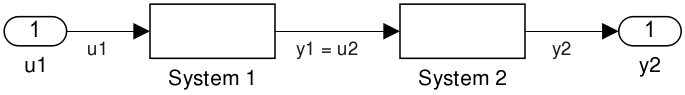
\includegraphics[scale=\modelscale]{schaltung_reihe.png}

    \item
    \textbf{Parallelschaltung}:\\
    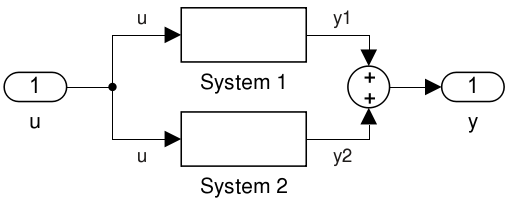
\includegraphics[scale=\modelscale]{schaltung_parallel.png}

    \item
    \textbf{gedämpftes Federpendel}:\\
    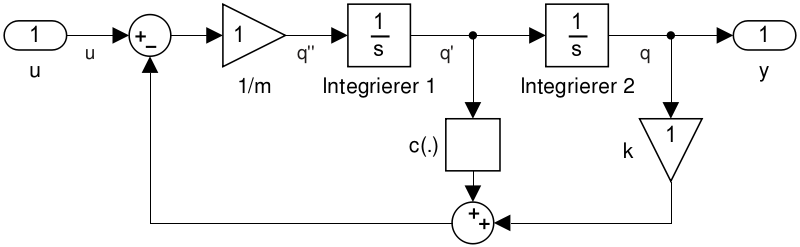
\includegraphics[scale=\modelscale]{federpendel_gedaempft.png}

    \item
    \textbf{allgemeines lineares System}:
    (in Simulink auch darstellbar durch einen \code{State-Space}- oder \code{LTI Systems}-Block,
    definiert durch $A, B, C, D$ bzw. ein \code{ss}-Objekt)\\
    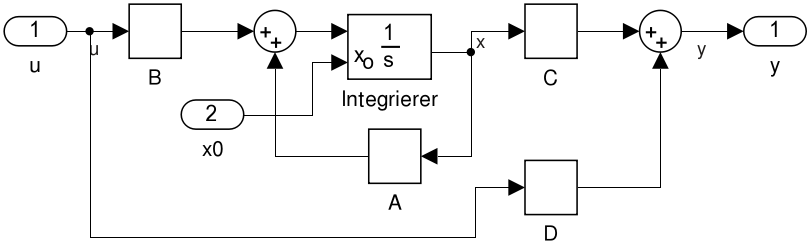
\includegraphics[scale=\modelscale]{lineares_system.png}
\end{itemize}

\pagebreak
